\section{Background estimation}
\label{sec:bckg}
The largest backgrounds in this dihiggs search at the end of selection are expected to come from $t \bar{t}$ and multi-jet production. The $t\bar{t}$ background is normalized using data while the multi-jet background is derived using a data-driven ABCD method as described in Sec. \ref{sec:multijet}. For all other backgrounds (diboson, $V$+jets, etc), Monte Carlo samples are used after normalizing their event yields to their expected cross sections and the appropriate integrated luminosity.

\subsection{Top normalisation and control region}
\label{subsec:topCR}
The \ttbar background normalization is calculated and validated using two dedicated control regions (CR). The first control region, CR1, is defined for the non-resonant and low-mass selections while the second, CR2, is defined for the high-mass selection. The definitions for CR1 and CR2 are given in Table \ref{tab:CRdef}. Tables \ref{tab:CR1}, \ref{tab:CR2}, and \ref{tab:CR3} show the number of observed and expected background events in the \mbb control region for the non-resonant, low-mass, and high-mass selections before the application of \ttbar normalization factors. The \mbb control region is orthogonal to the signal region due to the inversion of the \mbb cut.
\begin{table}
\begin{center}
\begin{tabular}{|c|c|c|}
\hline
 Variable 						&CR1 				& CR2 \\
\hline					
$m_{bb}$						& $m_{bb} < 100$ or $m_{bb} > 140$ & $m_{bb} < 100$ or $m_{bb} > 140$\\
$m_{WW}$ (GeV)   				& $<130$ 		 		& no-cut \\
$p_{\rm T}^{bb}$ (GeV) 			& $>150$ 		 		&$>350$\\
\hline
\end{tabular}
\end{center}
\caption{Definition of the kinematic regions used to normalise the Top background. $m_{bb} < 100$ or $m_{bb} > 140$ defines the sidebands in which the control regions are defined. Expected SM backgrounds compared to the measured data after each subsequent selection cut.} 
\label{tab:CRdef}
\end{table}

\begin{table}
  \begin{adjustbox}{width=1\textwidth}
    \begin{tabular}{l|c|c|c|c|c}
      \hline\hline
      \multicolumn{6}{c}{\textbf{CR}: \mbb Sideband non-resonant selection}\\\hline\hline
      Sample  	& $m_{WW}<130$ 	& $p_{\rm T}^{bb}>150$ 	& $p_{\rm T}^{bb}>230$ 	& $\Delta R_{bb}<1.2$  	& $\Delta R_{WW} <1.1$   \\\hline
      \ttbar 	& 23776.6 $\pm$ 87.2 	& 2370.9 $\pm$ 27.5 	& 363.8 $\pm$ 10.8 	& 114.3 $\pm$ 5.9 	& 91.7 $\pm$ 5.3 	\\\hline 
      QCD 	& 12587.3 $\pm$ 491.3 	& 1028.5 $\pm$ 147.5 	& 198.0 $\pm$ 73.3 	& 66.9 $\pm$ 34.6 	& 54.5 $\pm$ 29.2 \\\hline 
      W+jets 	& 3948.2 $\pm$ 31.2 	& 326.7 $\pm$ 6.2 	& 91.4 $\pm$ 2.9 	& 30.3 $\pm$ 1.7 	& 26.0 $\pm$ 1.6 	\\\hline 
      SingleTop 	& 1605.4 $\pm$ 18.0 	& 232.8 $\pm$ 6.6 	& 55.1 $\pm$ 3.3 	& 8.0 $\pm$ 1.3 	& 5.6 $\pm$ 1.1 		\\\hline 
      Dibosons 	& 109.9 $\pm$ 2.7 	& 17.6 $\pm$ 1.2 	& 6.5 $\pm$ 0.8 	& 3.9 $\pm$ 0.6 	& 2.7 $\pm$ 0.5 		\\\hline 
      Z+jets 	& 1107.6 $\pm$ 8.4 	& 66.9 $\pm$ 1.3 	& 18.7 $\pm$ 0.7 	& 5.1 $\pm$ 0.4 	& 4.2 $\pm$ 0.4 	\\\hline 
      \hline
      Background Sum 	& 43135.1$\pm$ 500.3 	& 4043.4$\pm$ 150.3 	& 733.5$\pm$ 74.2 	& 228.5$\pm$ 35.2 	& 184.6$\pm$ 29.7 	\\\hline 
      \hline
      XhhSM 	& 44.6 $\pm$ 2.2 	& 18.9 $\pm$ 1.2 	& 7.3 $\pm$ 0.6 	& 4.6 $\pm$ 0.5 	& 3.8 $\pm$ 0.4 	\\\hline 
      Data 	& 43199.0 	& 3947.0 	& 722.0 	& 220.0 	& 183.0 	\\\hline 
      \hline
    \end{tabular}
    \label{tab:CR1}
  \end{adjustbox}
  \caption{ The number of observed events and expected background events in the $m_{bb}$ side-bands for the non-resonant selection. The top CR is defined at the bbpt150 selection. No NF has been applied to the background yields. Only statistical uncertainties are shown.}
\end{table}

\begin{table}
  \begin{adjustbox}{width=1\textwidth}
    \begin{tabular}{l|c|c|c|c|c}
      \hline\hline
      \multicolumn{6}{c}{\textbf{CR}: \mbb Sideband low-mass selection}\\\hline\hline
      Sample  	& $m_{WW}<130$ 	& $p_{\rm T}^{bb}>150$ 	& $\Delta R_{bb}<1.1$  	& $\Delta R_{WW} <0.9$   & $630 < m_{hh} < 770$\\\hline
      \ttbar 	& 23776.6 $\pm$ 87.2 	& 2370.9 $\pm$ 27.5 	& 763.1 $\pm$ 15.8 	& 335.1 $\pm$ 10.6 	& 21.5 $\pm$ 2.6 		\\\hline 
      QCD 	& 12587.3 $\pm$ 491.3 	& 1028.5 $\pm$ 147.5 	& 336.8 $\pm$ 82.2 	& 146.8 $\pm$ 42.0 	& 21.9 $\pm$ 10.2 		\\\hline 
      W+jets 	& 3948.2 $\pm$ 31.2 	& 326.7 $\pm$ 6.2 	& 125.2 $\pm$ 3.7 	& 62.4 $\pm$ 2.6 	& 9.0 $\pm$ 0.9 		\\\hline 
      SingleTop 	& 1605.4 $\pm$ 18.0 	& 232.8 $\pm$ 6.6 	& 45.7 $\pm$ 3.1 	& 21.1 $\pm$ 2.1 	& 2.1 $\pm$ 0.7 		\\\hline 
      Dibosons 	& 109.9 $\pm$ 2.7 	& 17.6 $\pm$ 1.2 	& 8.4 $\pm$ 0.8 	& 4.3 $\pm$ 0.6 	& 0.6 $\pm$ 0.2 	\\\hline 
      Z+jets 	& 1107.6 $\pm$ 8.4 	& 66.9 $\pm$ 1.3 	& 11.7 $\pm$ 0.5 	& 8.5 $\pm$ 0.6 	& 2.1 $\pm$ 0.3 	\\\hline 
      \hline
      Background Sum 	& 43135.1$\pm$ 500.3 	& 4043.4$\pm$ 150.3 	& 1290.9$\pm$ 83.8 	& 578.3$\pm$ 43.5 	& 57.3$\pm$ 10.6 	\\\hline 
      \hline
      Xhh700 	& 4.2 $\pm$ 0.2 	& 3.2 $\pm$ 0.2 	& 1.8 $\pm$ 0.1 	& 1.5 $\pm$ 0.1 	& 0.7 $\pm$ 0.1 	\\\hline 
      Data 	& 43199.0 	& 3947.0 	& 1265.0 	& 543.0 	& 67.0	\\\hline 
      \hline
    \end{tabular}
    \label{tab:CR2}
  \end{adjustbox}
  \caption{ The number of observed events and expected background events in the $m_{bb}$ side-bands for the low-mass selection. The top CR is defined at the bbpt150 selection. To show how well the prediction matches data, no NF has been applied to any background. Only statistical uncertainties are shown.}
\end{table}

\begin{table}
  \begin{adjustbox}{width=1\textwidth}
    \begin{tabular}{l|c|c|c|c}
      \hline\hline
      \multicolumn{5}{c}{\textbf{CR}: \mbb Sideband high-mass selection}\\\hline\hline
      Sample  	& $p_{\rm T}^{bb}>350$  	& $p_{\rm T}^{WW}>360$  	& $\Delta R_{WW} <2.0$ 	& $1770 < m_{hh} < 2230$ 	 \\\hline
      \ttbar 	& 8568.7 $\pm$ 52.1 	& 5148.6 $\pm$ 40.4 	& 2099.1 $\pm$ 26.2 	& 327.6 $\pm$ 10.4 	\\\hline 
      QCD 	& 1298.7 $\pm$ 221.0 	& 679.5 $\pm$ 149.5 	& 444.0 $\pm$ 134.3 	& 74.4 $\pm$ 27.0 	\\\hline 
      W+jets 	& 2259.5 $\pm$ 7.9 	& 1556.2 $\pm$ 6.4 	& 804.1 $\pm$ 4.7 	& 142.3 $\pm$ 1.7 	\\\hline 
      SingleTop 	& 1778.1 $\pm$ 19.4 	& 1246.1 $\pm$ 16.2 	& 523.9 $\pm$ 10.6 	& 81.3 $\pm$ 4.1 	\\\hline 
      Dibosons 	& 170.6 $\pm$ 3.9 	& 115.0 $\pm$ 3.3 	& 57.4 $\pm$ 2.3 	& 8.8 $\pm$ 0.9 	\\\hline 
      Z+jets 	& 403.6 $\pm$ 2.1 	& 214.8 $\pm$ 1.4 	& 99.5 $\pm$ 1.0 	& 18.7 $\pm$ 0.4 	\\\hline 
      \hline
      Background Sum 	& 14479.1$\pm$ 228.1 	& 8960.0$\pm$ 155.9 	& 4028.0$\pm$ 137.4 	& 653.3$\pm$ 29.3	\\\hline 
      \hline
      Xhh2000 	& 25.7 $\pm$ 0.4 	& 21.7 $\pm$ 0.4 	& 12.1 $\pm$ 0.3 	& 5.1 $\pm$ 0.2 	\\\hline 
      Data 	& 14613.0 	& 8945.0 	& 4100.0 	& 698.0 	\\\hline 
      \hline
    \end{tabular}
  \end{adjustbox}
  \label{tab:CR3}
  \caption{ The number of observed events and expected background events in the $m_{bb}$ side-bands for the high-mass selection. The top CR is defined at the bbpt350 selection. No NF has been applied to the background yields. Only statistical uncertainties are shown.}
\end{table}

\begin{table}
\label{tab:NFs}
\begin{center}
\begin{tabular}{|c|c|c|c|}
%\hline
%\multicolumn{4}{c}{Top background normalisation factors in the two CRs} \\
\hline
Region & NF & $\sigma_{stat.}$ \\%& $\sigma_{syst.}$ \\
\hline
non-res and low-mass & 0.94 & 0.03 \\% & in progress\\
high-mass & 1.03 & 0.02 \\%& in progress\\
\hline
\end{tabular}
\end{center}
\caption{Normalisation factors for the two CRs, the statistical error includes only data statistics, the systematic error is shown to check the compatibility of the NF with one, but it is not directly used in the fit procedure.} 
\end{table}

The top normalization factors are determined by a simultaneous fit of signal and control regions, which include both top and QCD control regions~\ref{sec:multijet}. The factors differ between the low-mass and high-mass selections due to the different definitions of CR1 and CR2. The non-resonant selection shares CR1 and the \ttbar normalization with the low-mass selection. The normalization factors of the two top control regions are shown in Table \ref{tab:NFs}. Figures~\ref{fig:cr1_var} and ~\ref{fig:cr2_var} show distributions in CR1 and CR2 for the variables used in event selection.

\begin{figure}[!h]
\begin{center}
\includegraphics*[width=0.47\textwidth] {chapters/dihiggs2/figures/ControlPlots/36ifb_CPUpdated_opt700_mBBcr_plots_094/C_mBBcr_opt700ichep_mww_bbpt150_WWMass_regionA_met25d020}
\includegraphics*[width=0.47\textwidth] {chapters/dihiggs2/figures/ControlPlots/36ifb_CPUpdated_opt700_mBBcr_plots_094/C_mBBcr_opt700ichep_mww_bbpt150_bbPt_regionA_met25d020}
\includegraphics*[width=0.47\textwidth] {chapters/dihiggs2/figures/ControlPlots/36ifb_CPUpdated_opt700_mBBcr_plots_094/C_mBBcr_opt700ichep_mww_bbpt150_drbb_regionA_met25d020}
\includegraphics*[width=0.47\textwidth] {chapters/dihiggs2/figures/ControlPlots/36ifb_CPUpdated_opt700_mBBcr_plots_094/C_mBBcr_opt700ichep_mww_bbpt150_drww_regionA_met25d020}
\includegraphics*[width=0.47\textwidth] {chapters/dihiggs2/figures/ControlPlots/36ifb_CPUpdated_opt700_mBBcr_plots_094/C_mBBcr_opt700ichep_mww_bbpt150_bbMass_regionA_met25d020}
\includegraphics*[width=0.47\textwidth] {chapters/dihiggs2/figures/ControlPlots/36ifb_CPUpdated_opt700_mBBcr_plots_094/C_mBBcr_opt700ichep_mww_bbpt150_hhMass_regionA_met25d020}
\caption[Event selection variables in CR1 for the non-resonant and low-mass selections.]{Event selection variables in CR1 for the non-resonant and low-mass selections. \ttbar NFs as described in~\ref{subsec:topCR} have been applied The uncertainties shown include the statistical and systematic uncertainties described in ~\ref{sec:syst}.}
\label{fig:cr1_var}
\end{center}
\end{figure}


\begin{figure}[!h]
\begin{center}
\includegraphics*[width=0.47\textwidth] {chapters/dihiggs2/figures/ControlPlots/36ifb_CPUpdated_opt2000_mBBcr_plots_103/C_mBBcr_opt2000ichep_bbpt350_WWMass_regionA_met25d020}
\includegraphics*[width=0.47\textwidth] {chapters/dihiggs2/figures/ControlPlots/36ifb_CPUpdated_opt2000_mBBcr_plots_103/C_mBBcr_opt2000ichep_bbpt350_bbPt_regionA_met25d020}
\includegraphics*[width=0.47\textwidth] {chapters/dihiggs2/figures/ControlPlots/36ifb_CPUpdated_opt2000_mBBcr_plots_103/C_mBBcr_opt2000ichep_bbpt350_WWPt_regionA_met25d020}
\includegraphics*[width=0.47\textwidth] {chapters/dihiggs2/figures/ControlPlots/36ifb_CPUpdated_opt2000_mBBcr_plots_103/C_mBBcr_opt2000ichep_bbpt350_drww_regionA_met25d020}
\includegraphics*[width=0.47\textwidth] {chapters/dihiggs2/figures/ControlPlots/36ifb_CPUpdated_opt2000_mBBcr_plots_103/C_mBBcr_opt2000ichep_bbpt350_bbMass_regionA_met25d020}
\includegraphics*[width=0.47\textwidth] {chapters/dihiggs2/figures/ControlPlots/36ifb_CPUpdated_opt2000_mBBcr_plots_103/C_mBBcr_opt2000ichep_bbpt350_hhMass_regionA_met25d020}
\caption[Event selection variables in CR2 for the high-mass selection.]{Event selection variables in CR2 for the non-resonant and low-mass selections. \ttbar NFs as described in~\ref{subsec:topCR} have been applied The uncertainties shown include the statistical and systematic uncertainties described in ~\ref{sec:syst}.}
\label{fig:cr2_var}
\end{center}
\end{figure}

\subsection{Multi-jet background}
\label{sec:multijet}
Multi-jet backgrounds can enter in the event selection if a jet %from heavy flavour decays 
is mis-identified as an electron or a muon and used as a lepton in the analysis. Such phenomena are not accurately reproduced by MC simulation due to the large uncertainties in the jet shower shape simulation and uncertainties in jet fragmentation functions and kinematics. In order to estimate the contributions of multi-jet processes, a data-driven ABCD method is used to estimate this background in the present analysis.
%%Such methods are used extensively in the top group analyses.

The ABCD method uses three control regions (the B, C, and D regions) to estimate the contribution of a given background in the signal (A) region. Cuts on two ideally
uncorrelated variables are used to create the signal and various control regions, e.g. the A region passes both cuts, the B and C regions each pass one cut and fail the other, while the D region fails both cuts. The absolute value of the significance of the lepton impact parameter, \dsig, and the missing transverse energy (MET) are used as the two variables used to define the regions in the ABCD method for this analysis. The correlation between MET and \dsig was tested using \ttbar MC, and the two variables were found to be negligibly correlated (correlation factor $\sim\mathcal{O}(10^{-2}$) at all stages of event selection. The regions are thus defined 
\begin{itemize}
\item A region: MET $>$ 25 GeV, \dsig $<$ 2.0
\item B region: MET $<$ 25 GeV, \dsig $<$ 2.0
\item C region: MET $>$ 25 GeV, \dsig $>$ 2.0
\item D region: MET $<$ 25 GeV, \dsig $>$ 2.0
\end{itemize}
Figure~\ref{fig:abcdCartoon} shows a pictoral representation of the four regions.
\begin{figure}[h!]
\begin{center}
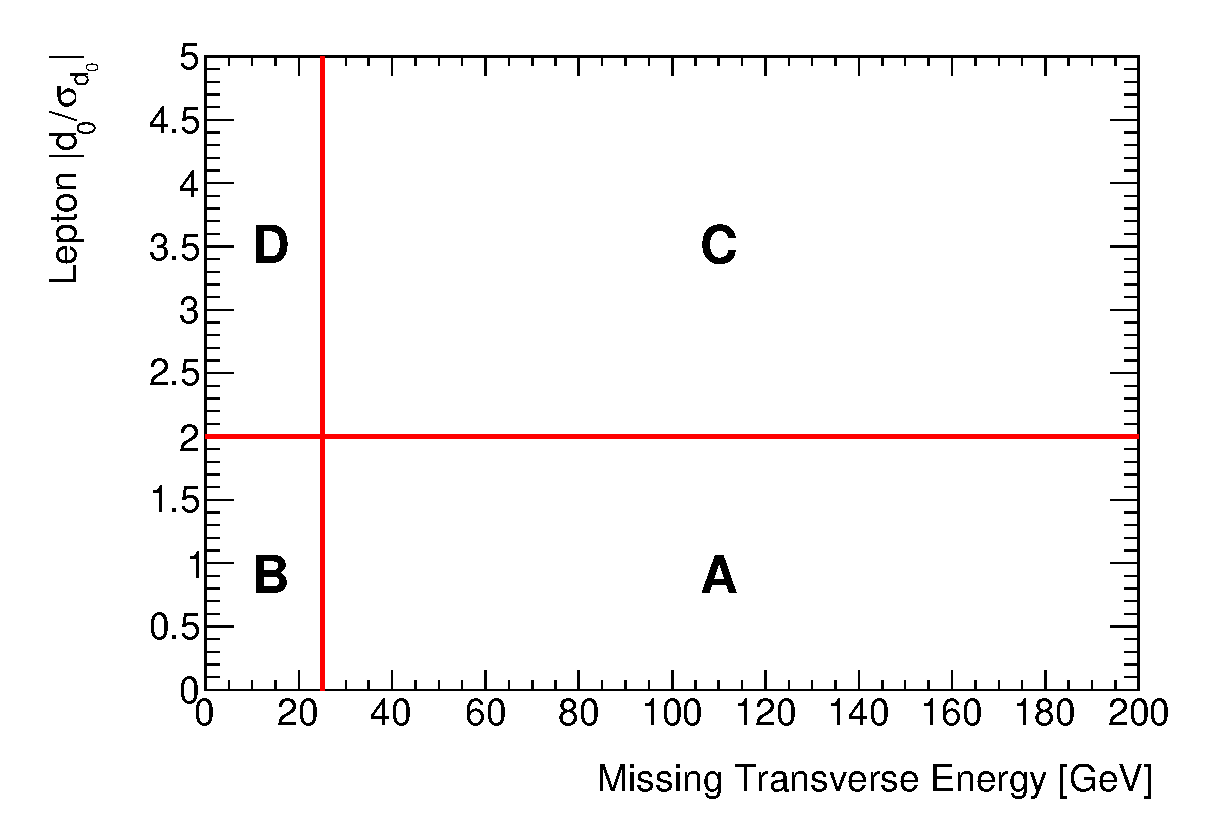
\includegraphics[width=0.6\textwidth]{chapters/dihiggs2/figures/abcdExample_met_vs_d0sigBL20}
\end{center}
\label{fig:abcdCartoon}
\caption{A pictoral representation of the four regions used in the ABCD calculation.}
\end{figure}

Assuming that the two variables chosen to define the ABCD regions are completely uncorrelated, the yield of the process being modeled (QCD multi-jets in this case) in the A region is given by \begin{equation}
N_{A} = N_C \frac{N_B}{N_D}
\label{eq:simpleABCD}
\end{equation}
where the yields $N_i$ are yields calculated from data - all Monte Carlo backgrounds (\ttbar, W/Z+jets, single top, diboson processes) in region $i$ ($N_i = N_i^{\text{data}} - N_i^{\text{MC Bkgs}}$). The assumption underlying Equation~\ref{eq:simpleABCD} is that the relationship between the yields in the B and D regions is the same as the relationship between the A and C regions, i.e. 
\begin{equation}
\frac{N_{A}}{N_{C}} = \frac{N_B}{N_D}
\label{eq:correlationStatement}
\end{equation}
Using equation ~\ref{eq:correlationStatement}, the quantity $R= \frac{N_{C} N_B}{N_{A} N_D}$ can be defined. In the case of two completely uncorrelated variables, $R=1$ and the ABCD estimation reduces to Equation~\ref{eq:simpleABCD}. If the two variables are not completely uncorrelated, the $R$ factor enters as a correction to Equation~\ref{eq:simpleABCD} for the multi-jet estimation in the A region, and the expression can be rewritten as
\begin{equation}
N_{A} = R \frac{N_C N_B}{N_D}
\label{eq:advancedABCD}
\end{equation}
The $R$ factor is calculated for each selection (non-resonant, low mass, and high mass) individually, and the results at each cut in each selection is provided in Table~\ref{tab:rValues}.

\begin{table}[h!]
\centering
\begin{tabular}{c|c|c|c|c}
\hline\hline
\multicolumn{5}{c}{QCD $R$ Values, Non-resonant Selection}\\\hline\hline
mww     & bbpt150       & bbpt230       & drbb12        & drww11        \\\hline
0.74 $\pm$ 0.03 	& 0.67 $\pm$ 0.10 	& 0.67 $\pm$ 0.24 	& 0.57 $\pm$ 0.33 	& 0.20 $\pm$ 0.19	\\\hline 
\end{tabular}

\begin{tabular}{c|c|c|c|c}
\multicolumn{5}{c}{QCD $R$ Values, Low Mass Selection}\\\hline\hline
mww     & bbpt150       & drbb11        & drww09        & hh700 \\\hline
0.74 $\pm$ 0.03 	& 0.67 $\pm$ 0.10 	& 0.67 $\pm$ 0.18 	& 0.28 $\pm$ 0.15 	& 0.19 $\pm$ 0.72	\\\hline 
\hline\hline
\end{tabular}

\begin{tabular}{c|c|c|c}
\multicolumn{4}{c}{QCD $R$ Values, High Mass Selection}\\\hline\hline
bbpt350         & wwpt360       & drww20        & hh2000above   \\\hline
0.47 $\pm$ 0.09 	& 0.43 $\pm$ 0.11 	& 0.46 $\pm$ 0.15 	& 1.05 $\pm$ 0.89	\\\hline 
\hline\hline
\end{tabular}


\caption{Values calculated for $R$ at each stage in the non-resonant,
  low mass, and high mass selections. The estimate of multi-jet
  contribution in the A region uses the $R$ value calculated after the
  first cut of each selection.} \label{tab:rValues}
\end{table}
In order to minimize the dependence of $R$ from the event selection cuts, the $R$ value calculated after the first cut of each selection (0.74 and 0.47) is used in Equation~\ref{eq:advancedABCD} to estimate the multi-jet background after each subsequent cut. Once the normalization of the multi-jet background in the A region is calculated using Equation~\ref{eq:advancedABCD}, the shape of the multi-jet template is taken from the data - Monte Carlo distribution in the C region since the two are kinematically identical except for the cut on \dsig.

The uncertainty due to the limited statistics in the B and D regions is the main source of the multi-jet estimation method systematics. In order to minimize this error, the yields from the  B and D regions used in the ABCD calculation are frozen at a level of the cutflow to minimize statistical fluctuations. The B and D region yields are frozen after the \ptbb $>$ 230 GeV cut for the non-resonant selection, after the \drbb $<$ 1.1 cut for the low mass selection, and after the \drww $<$ 2.0 cut for the high mass selection. %Appendix~\ref{app:qcd_BDregionStudy_appendix} details the study carried out to select the stage at which to freeze the B and D regions. 

Since \ttbar and  multi-jet events contaminate the control regions used for their estimation, additional studies were performed via an iterative procedure to ensure that the \ttbar and QCD yields converge to stable values and that the estimation technique is able to disentangle between the two backgrounds. The iterative procedure begins with the QCD estimate set to zero and continues as follows:
\begin{enumerate}
\item Calulate \ttbar NF at appropriate cut \textbf{before} QCD is calculated
\item Start at beginning of cutflow, apply \ttbar NF, and calculate QCD
\item Move through cutflow to \ttbar NF cut
\item Calculate new \ttbar NF
\item Repeat steps 2 - 4
\end{enumerate}
If the procedure converges, the estimate is said to be stable. Tables~\ref{tab:ttbarQCDiter_nonres},~\ref{tab:ttbarQCDiter_low}, and~\ref{tab:ttbarQCDiter_high} show the iterations for the non-resonant, low mass, and high mass selections. Iteration 0 starts with zero QCD in the background estimate. Yields are provided for QCD and \ttbar after the first selection cut (noted as sample\_first) and in the final \mbb signal region (noted as sample\_SR). The QCD yield at the \ttbar normalization cut is also provided. The final column shows the calculated normalization factor for \ttbar. For all selections, convergence (change in \ttbar normalization $<$5\%) is observed after just a few iterations for all selections. 
\begin{center}
\begin{table}[h!]%\fontsize{9}{10}\selectfont
  \begin{tabular}{l|c|c|c|c|c|c}
    \hline\hline
    Iteration &      nQCD\_first &   n\_QCD\_nf &    nQCD\_SR &      ttbar\_first &           ttbar\_SR &     ttbarNF       \\\hline
    0        &       0.00 &          0.00 &          0.00 &          24637.64 &      65.92 &         1.43 $\pm$ 0.02  \\\hline
    1        &       4226.57 &       273.95 &        3.30 &          35249.05 &      94.31 &         0.92 $\pm$ 0.02   \\\hline
    2        &       15765.74 &      1381.06 &       19.04 &         22708.20 &      60.75 &         0.94 $\pm$ 0.03   \\\hline
    3        &       15311.64 &      1335.16 &       18.33 &         23145.35 &      61.92 &         0.94 $\pm$ 0.03   \\\hline
    \hline
  \end{tabular}
\caption{Iteration of \ttbar normalization and QCD estimate for the non-resonant selection. The '\_first' region is defined after the \mww $<$ 130 GeV cut and the '\_nf' region is defined after requiring \ptbb $>$ 150 GeV. Convergence is observed after two iterations.}
\label{tab:ttbarQCDiter_nonres}
\end{table}

\begin{table}[h!]%\fontsize{9}{10}\selectfont
  \begin{tabular}{l|c|c|c|c|c|c}
    \hline\hline
    Iteration &      nQCD\_first &   n\_QCD\_nf &    nQCD\_SR &      ttbar\_first &           ttbar\_SR &     ttbarNF       \\\hline
    0        &       0.00 &          0.00 &          0.00 &          24637.64 &      11.28 &         1.43 $\pm$ 0.02        \\\hline
    1        &       4226.57 &       273.95 &        1.13 &          35249.05 &      16.14 &         0.92 $\pm$ 0.02        \\\hline
    2        &       15765.74 &      1381.06 &       8.14 &          22708.20 &      10.40 &         0.94 $\pm$ 0.03        \\\hline
    3        &       15311.64 &      1335.16 &       7.81 &          23145.35 &      10.60 &         0.94 $\pm$ 0.03        \\\hline
    \hline
  \end{tabular}
\caption{Iteration of \ttbar normalization and QCD estimate for the low mass selection. The '\_first' region is defined after the \mww $<$ 130 GeV cut and the '\_nf' region is defined after requiring \ptbb $>$ 150 GeV. Convergence is observed after two iterations.}
\label{tab:ttbarQCDiter_low}
\end{table}

\begin{table}[h!]%\fontsize{9}{10}\selectfont
  \begin{tabular}{l|c|c|c|c|c|c}
    \hline\hline
    Iteration &      nQCD\_first &   n\_QCD\_nf &    nQCD\_SR &      ttbar\_first &           ttbar\_SR &     ttbarNF       \\\hline
    0        &       0.00 &          0.00 &          0.00 &          8810.24 &       6.70 &          1.26 $\pm$ 0.02        \\\hline
    1        &       92.73 &         40.56 &         0.11 &          11133.25 &      8.47 &          0.99 $\pm$ 0.02        \\\hline
    2        &       1595.54 &       541.28 &        1.40 &          8679.56 &       6.60 &          1.03 $\pm$ 0.03        \\\hline
    3        &       1238.18 &       432.83 &        1.12 &          9063.72 &       6.90 &          1.03 $\pm$ 0.02        \\\hline
    \hline
  \end{tabular}
\caption{Iteration of \ttbar normalization and QCD estimate for the low mass selection. The '\_first' region is defined after the \ptbb $>$ 350 GeV cut and the '\_nf' region is defined after requiring \ptww $>$ 360 GeV. Convergence is observed after two iterations.}
\end{table}
\label{tab:ttbarQCDiter_high}
\end{center}

Since the \mtw distribution should contain a large multi-jet contribution at low \mtw, the agreement between data and prediction in the \mtw distribution for each selection acts as a closure test on the estimation of the multi-jet background by the ABCD method. Figure~\ref{fig:qcdMtW} shows the \mtw distributions in CR1 and CR2. Good agreement is observed.

\begin{figure}[!h]
\begin{center}
\includegraphics*[width=0.47\textwidth] {chapters/dihiggs2/figures/ControlPlots/36ifb_CPUpdated_opt700_mBBcr_plots_094/C_mBBcr_opt700ichep_mww_bbpt150_wlepmtben_regionA_met25d020}
\includegraphics*[width=0.47\textwidth] {chapters/dihiggs2/figures/ControlPlots/36ifb_CPUpdated_opt2000_mBBcr_plots_103/C_mBBcr_opt2000ichep_bbpt350_wlepmtben_regionA_met25d020}
\caption[Transverse leptonic $W$ mass plots in CR1 and CR2.]{Transverse leptonic $W$ mass plots in CR1 and CR2. \ttbar NFs as described in~\ref{subsec:topCR} have been applied The percent uncertainties shown in the bottom of each plot include the statistical and systematic uncertainties described in ~\ref{sec:syst}.}
\label{fig:qcdMtW}
\end{center}
\end{figure}

To evaluate the systematic error of the estimation, a Sherpa multi-$b$-jet sample is used to compare the ABCD prediction to the Monte Carlo expectation using events with exactly one lepton and four jets. No $b$-tagging requirements or other event selection cuts are applied. Pseudo-data is produced using the multi-jet Monte Carlo and events from the nominal \ttbar Monte Carlo. The $R$ factor is calculated using the inclusive $b$-tag (0, 1, or 2 $b$-tags) and used to estimate the QCD contribution in the two $b$-tag exclusive region. The percent difference between the number of events from the ABCD estimation and the number of multi-jet events from Monte Carlo used to produce the pseudo-data is taken as the systematic uncertainty. This uncertainty is calculated to be 36\%.

%validated using the observed $m_{\rm T}$ distribution in events in the
%top control region with one $b$-tag, as shown in
%Figure~\ref{fig:mwt}.
%\begin{figure}
%\begin{center}
%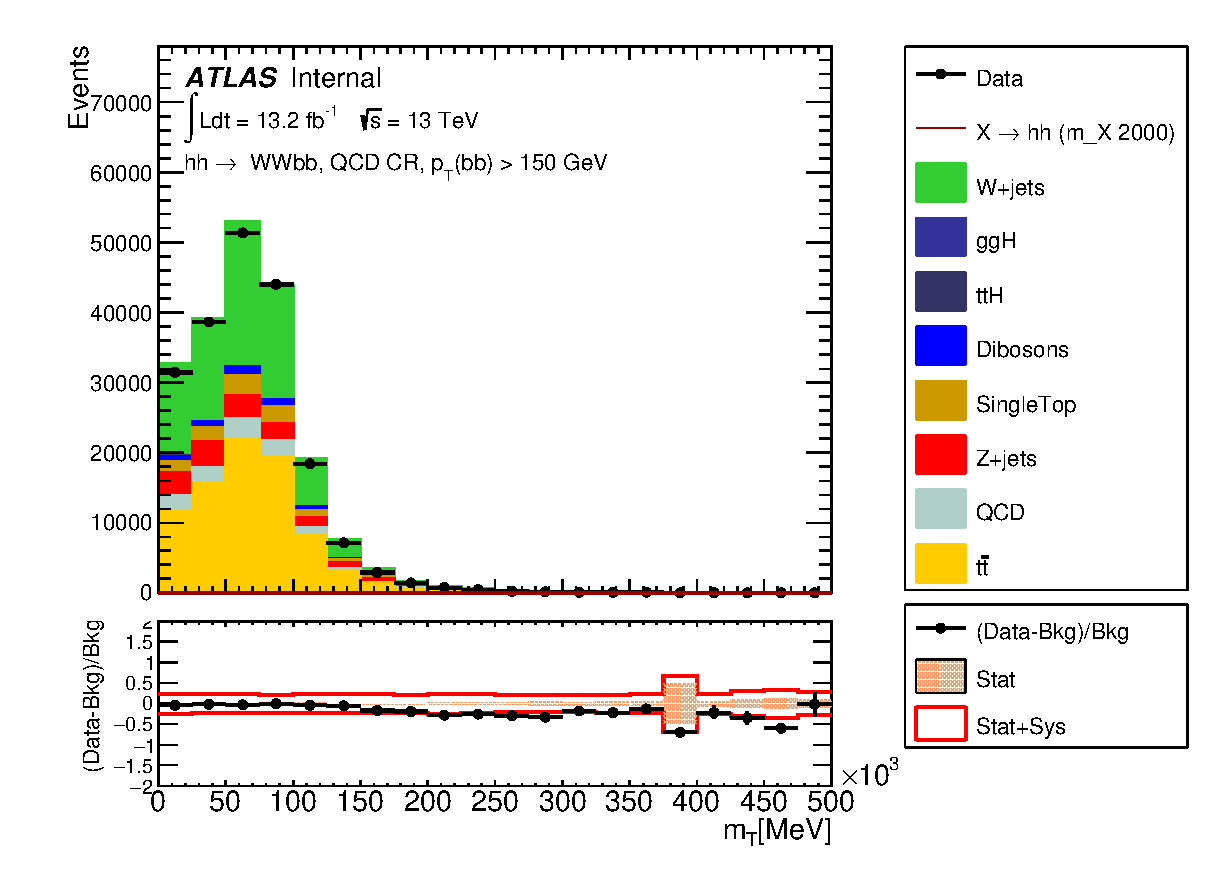
\includegraphics[width=0.47\textwidth, height=0.35\textwidth]{figures/C_bj1_opt700_bbpt150_wlepmtben.eps}
%\includegraphics[width=0.47\textwidth, height=0.35\textwidth]{figures/ControlPlots/CR1/C_opt700_bbpt150_wlepmtben.eps}
%\end{center}
%\caption{$m_{\rm T}$ distribution for events in the QCD enriched control region
%   with one $b$-tag (left) and with $t\bar{t}$ control region two $b$-tag (right).}
%\label{fig:mwt}
%\end{figure}













